\documentclass[11pt,a4paper]{article}

% Pacotes essenciais
\usepackage[utf8]{inputenc}
\usepackage[T1]{fontenc}
\usepackage{lmodern}
\usepackage[portuguese]{babel}
\usepackage{graphicx}
\usepackage{amsmath}
\usepackage{amsfonts}
\usepackage{amssymb}
\usepackage{float}
\usepackage{caption}
\usepackage{subcaption}
\usepackage{xcolor}
\usepackage{colortbl}
\usepackage{fancyhdr}
\usepackage{geometry}
\usepackage{titlesec}
\usepackage{lipsum}
\usepackage[alf]{abntex2cite}
\usepackage{booktabs}
\usepackage{array}
\usepackage{enumitem}
\usepackage{tikz}
\usetikzlibrary{shapes.geometric}
\usepackage[hidelinks]{hyperref}

% Definição das cores
\definecolor{headercolor}{HTML}{b11116}
\definecolor{secondarycolor}{HTML}{3a5461}

% Configuração da página
\geometry{
    a4paper,
    top=2.8cm,
    bottom=2.5cm,
    left=2.5cm,
    right=2.5cm,
    headheight=1.2cm,
    headsep=0.5cm
}

% Configuração do cabeçalho
\pagestyle{fancy}
\fancyhf{}
\renewcommand{\headrulewidth}{0pt}
\renewcommand{\footrulewidth}{0.5pt}

\fancyhead[L]{%
    \begin{tikzpicture}[remember picture, overlay]
        \fill[headercolor] (current page.north west) rectangle ([yshift=-1.2cm]current page.north east);
        \node[anchor=west, inner sep=0pt] at ([xshift=1cm, yshift=-0.6cm]current page.north west) 
            {
\includegraphics[height=0.8cm]{imgs/base/fatec-rgt.png}};
        \node[anchor=east, inner sep=0pt] at ([xshift=-1cm, yshift=-0.6cm]current page.north east) 
            {
\includegraphics[height=0.9cm]{imgs/base/cps-logo.png}};
        \node[anchor=east, inner sep=0pt] at ([xshift=-2.8cm, yshift=-0.6cm]current page.north east) 
            {
\includegraphics[height=1.05cm]{imgs/base/governo-sp-secretaria-logo.png}};
    \end{tikzpicture}
}

\fancyfoot[L]{\footnotesize\textcolor{secondarycolor}{Faculdade de Tecnologia do Estado de São Paulo\\ fatecregistro.cps.sp.gov.br}}
\fancyfoot[R]{\thepage}

% Configuração dos títulos das seções
\titleformat{\section}
    {\normalfont\large\bfseries\color{secondarycolor}}
    {\thesection}{1em}{}

\titleformat{\subsection}
    {\normalfont\normalsize\bfseries\color{secondarycolor}}
    {\thesubsection}{1em}{}

\begin{document}

% ===== CAPA =====
\begin{titlepage}
    \centering
    
    % Logos no topo
    \begin{tikzpicture}[remember picture, overlay]
        \fill[headercolor] (current page.north west) rectangle ([yshift=-1.2cm]current page.north east);
        \node[anchor=west, inner sep=0pt] at ([xshift=1cm, yshift=-0.6cm]current page.north west) 
            {
\includegraphics[height=0.8cm]{imgs/base/fatec-rgt.png}};
        \node[anchor=east, inner sep=0pt] at ([xshift=-1cm, yshift=-0.6cm]current page.north east) 
            {
\includegraphics[height=0.9cm]{imgs/base/cps-logo.png}};
        \node[anchor=east, inner sep=0pt] at ([xshift=-2.8cm, yshift=-0.6cm]current page.north east) 
            {
\includegraphics[height=1.05cm]{imgs/base/governo-sp-secretaria-logo.png}};
    \end{tikzpicture}
    
    \vspace*{3.5cm}
    
    % Nome da faculdade
    {\normalsize FACULDADE DE TECNOLOGIA DO ESTADO DE SÃO PAULO\par}
    \vspace{0.5cm}
    
    % Curso
    {\normalsize DESENVOLVIMENTO DE SOFTWARE MULTIPLATAFORMA\par}
    
    \vspace{4cm}
    
    % Artefatos do Projeto de Software
    {\normalsize ARTEFATOS DO PROJETO DE SOFTWARE\par}
    
    \vspace{0.3cm}
    
    % Nome do projeto
    {\normalsize Análise Computacional de Sistemas Complexos Utilizando Métodos Numéricos Avançados\par}
    
    \vspace{3cm}
    
    % Autores
    {\normalsize
    João da Silva\\
    Maria Santos\\
    Pedro Oliveira
    }
    
    \vfill
    
    % Rodapé
    {\small Registro -- SP\\
    2026}
    
\end{titlepage}

% Força o cabeçalho em todas as páginas
\pagestyle{fancy}

% ===== SUMÁRIO =====
\tableofcontents
\newpage

% ===== NOTA IMPORTANTE =====
\section*{Nota Importante sobre os Artefatos}

\noindent Este documento apresenta exemplos de como inserir os principais artefatos de um projeto de software. Todos os artefatos podem ser inseridos de duas formas:

\begin{enumerate}
    \item \textbf{Como imagens:} Criar os artefatos em ferramentas externas (Canva, Miro, Draw.io, Figma, etc.) e inserir como imagens PNG/JPG usando o comando \texttt{\textbackslash includegraphics}
    \item \textbf{Como código LaTeX:} Usar tabelas e diagramas TikZ diretamente no documento (exemplos fornecidos)
\end{enumerate}

\subsection*{Lista de Artefatos e suas Finalidades}

\begin{itemize}
    \item \textbf{CANVAS:} Modelo de negócio e estratégia
    \item \textbf{SWOT:} Análise estratégica de forças, fraquezas, oportunidades e ameaças
    \item \textbf{UX/UI:} Design de interface e experiência do usuário
    \item \textbf{Website:} Estrutura e especificações técnicas web
    \item \textbf{Diagramas UML:} Modelagem visual do sistema
    \item \textbf{DevOps:} Infraestrutura, automação e práticas de entrega contínua
\end{itemize}

\vspace{0.5cm}
\noindent\rule{\textwidth}{0.5pt}

\newpage

% ===== CANVAS =====
\section{CANVAS: Modelo de Negócio e Estratégia}

O Business Model Canvas \cite{santos2024} é uma ferramenta visual estratégica\footnote{O Canvas foi desenvolvido por Alexander Osterwalder e é amplamente utilizado em startups e empresas estabelecidas para modelagem de negócios.} que permite descrever, analisar e projetar modelos de negócio de forma clara e objetiva. O canvas é dividido em nove blocos fundamentais que cobrem as principais áreas de um negócio.

\subsection{Como Inserir o CANVAS}

Para inserir o modelo Canvas no projeto, você pode utilizar tabelas ou imagens. Abaixo um exemplo de estrutura básica:

\begin{table}[H]
\centering
\caption{Business Model Canvas -- Visão Geral}
\label{tab:canvas}
\small
\begin{tabular}{|p{2.5cm}|p{2.5cm}|p{2.8cm}|p{2.5cm}|p{2.8cm}|}
\hline
\textbf{Parcerias Principais} & \textbf{Atividades Chave} & \textbf{Proposta de Valor} & \textbf{Relacionamento} & \textbf{Segmentos} \\
\hline
Fornecedores, parceiros, provedores cloud & Desenvolvimento, manutenção, análise & Automação, redução de custos, interface intuitiva & Suporte, treinamentos, portal & PMEs, comercial, administrativo \\
\hline
\multicolumn{2}{|p{5.5cm}|}{\textbf{Estrutura de Custos}} & \multicolumn{3}{p{7.5cm}|}{\textbf{Fontes de Receita}} \\
\hline
\multicolumn{2}{|p{5.5cm}|}{Desenvolvimento, infraestrutura, marketing, equipe} & \multicolumn{3}{p{7.5cm}|}{Licenças mensais/anuais, customização, suporte premium, treinamentos} \\
\hline
\end{tabular}
\end{table}

\textbf{Dica:} Você também pode criar o Canvas em ferramentas como Canva, Miro ou PowerPoint e inserir como imagem:

\begin{verbatim}
\begin{figure}[H]
\centering
\includegraphics[width=\textwidth]{imgs/canvas-modelo.png}
\caption{Business Model Canvas do Projeto}
\label{fig:canvas}
\end{figure}
\end{verbatim}

% ===== SWOT =====
\section{SWOT: Análise Estratégica}

A Análise SWOT (Strengths, Weaknesses, Opportunities, Threats) ou FOFA (Forças, Oportunidades, Fraquezas e Ameaças) \cite{oliveira2023} é uma ferramenta fundamental para planejamento estratégico\footnote{A análise SWOT foi criada na década de 1960 por Albert Humphrey no Stanford Research Institute.} que permite identificar fatores internos e externos que impactam o projeto. Analisa forças, fraquezas, oportunidades e ameaças do projeto.

\subsection{Como Inserir a Análise SWOT}

A matriz SWOT pode ser apresentada em formato de tabela conforme o exemplo abaixo:

\begin{table}[H]
\centering
\caption{Análise SWOT do Projeto}
\label{tab:swot}
\begin{tabular}{|p{7.2cm}|p{7.2cm}|}
\hline
\multicolumn{2}{|c|}{\cellcolor{secondarycolor!20}\textbf{FATORES INTERNOS}} \\
\hline
\textbf{FORÇAS (Strengths)} & \textbf{FRAQUEZAS (Weaknesses)} \\
\hline
\begin{minipage}[t]{7cm}
\begin{itemize}
    \item Equipe técnica qualificada
    \item Tecnologia moderna e escalável
    \item Interface intuitiva e amigável
    \item Baixo custo de implementação
    \item Suporte técnico especializado
    \item Integração com sistemas existentes
\end{itemize}
\end{minipage}
&
\begin{minipage}[t]{7cm}
\begin{itemize}
    \item Marca pouco conhecida no mercado
    \item Recursos financeiros limitados
    \item Dependência de fornecedores externos
    \item Equipe de vendas reduzida
    \item Documentação incompleta
    \item Testes automatizados insuficientes
\end{itemize}
\end{minipage}
\\
\hline
\multicolumn{2}{|c|}{\cellcolor{secondarycolor!20}\textbf{FATORES EXTERNOS}} \\
\hline
\textbf{OPORTUNIDADES (Opportunities)} & \textbf{AMEAÇAS (Threats)} \\
\hline
\begin{minipage}[t]{7cm}
\begin{itemize}
    \item Crescimento do mercado de SaaS
    \item Digitalização de empresas
    \item Programas de incentivo fiscal
    \item Parcerias com universidades
    \item Demanda por automação
    \item Expansão para novos nichos
\end{itemize}
\end{minipage}
&
\begin{minipage}[t]{7cm}
\begin{itemize}
    \item Concorrência com players consolidados
    \item Mudanças na legislação
    \item Crises econômicas
    \item Vulnerabilidades de segurança
    \item Rápida obsolescência tecnológica
    \item Resistência à mudança dos usuários
\end{itemize}
\end{minipage}
\\
\hline
\end{tabular}
\end{table}

\subsection{Recomendações Estratégicas}

Com base na análise SWOT, as principais estratégias devem focar em:
\begin{itemize}
    \item \textbf{Forças + Oportunidades:} Investir no marketing digital para aproveitar o crescimento do mercado
    \item \textbf{Forças + Ameaças:} Reforçar a segurança para se diferenciar da concorrência
    \item \textbf{Fraquezas + Oportunidades:} Buscar parcerias para ampliar a presença no mercado
    \item \textbf{Fraquezas + Ameaças:} Criar planos de contingência e melhorar a documentação
\end{itemize}

% ===== UX/UI =====
\section{UX/UI: Design de Interface e Experiência do Usuário}

UX (User Experience) e UI (User Interface) \cite{silva2025} são disciplinas complementares focadas em criar produtos digitais que sejam funcionais, acessíveis e agradáveis de usar.\footnote{Ferramentas populares para design UX/UI incluem Figma, Adobe XD, Sketch e InVision.} O UX concentra-se na experiência geral do usuário, enquanto o UI cuida dos elementos visuais e interativos.

\subsection{Como Inserir Mockups e Protótipos}

Os artefatos de UX/UI geralmente incluem wireframes, mockups e protótipos que podem ser inseridos como imagens:

\begin{figure}[H]
\centering
\begin{minipage}{0.45\textwidth}
    \centering
    \fbox{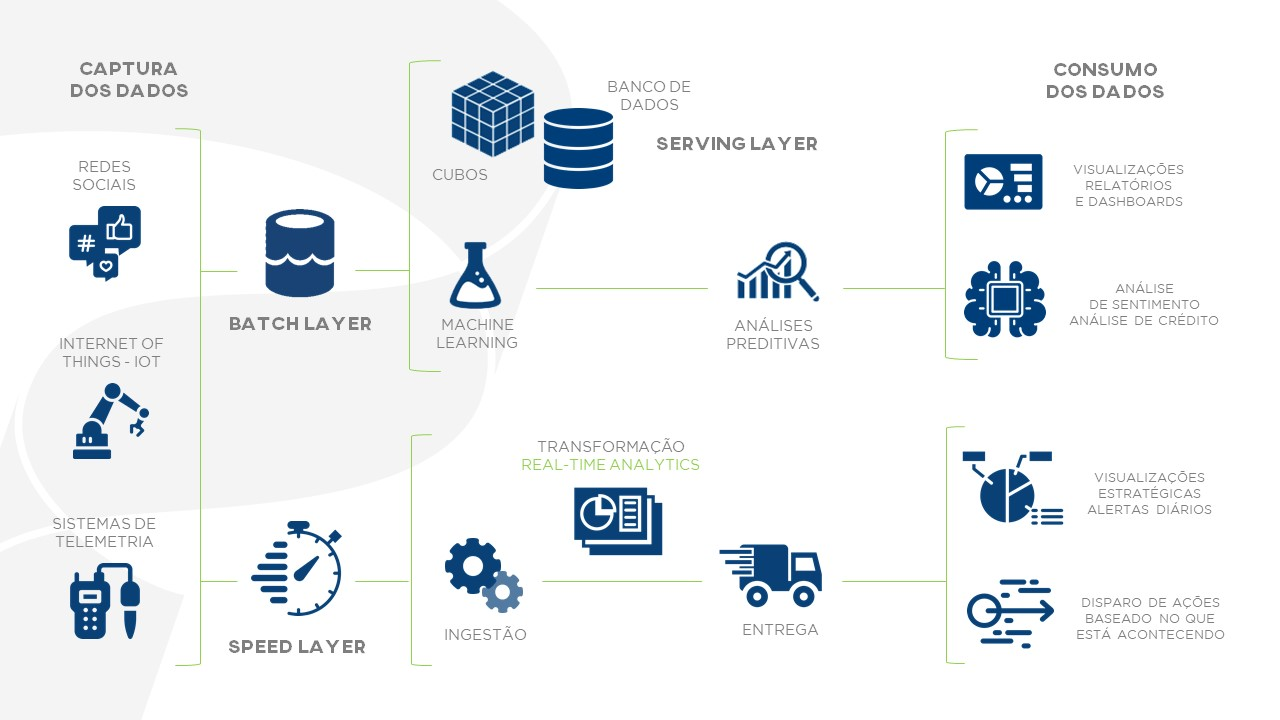
\includegraphics[width=0.9\textwidth]{imgs/img_001.jpg}}
    \caption{Wireframe da tela inicial}
    \label{fig:wireframe}
\end{minipage}
\hfill
\begin{minipage}{0.45\textwidth}
    \centering
    \fbox{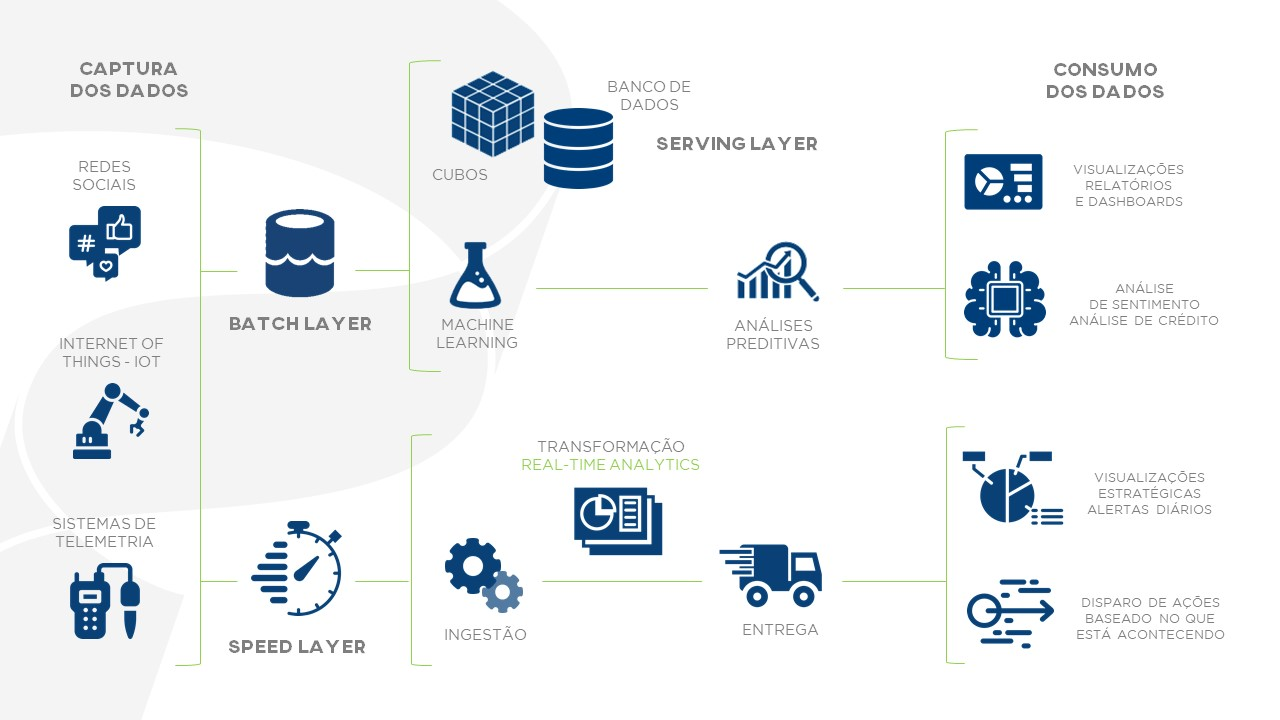
\includegraphics[width=0.9\textwidth]{imgs/img_001.jpg}}
    \caption{Mockup de alta fidelidade}
    \label{fig:mockup}
\end{minipage}
\end{figure}

\subsection{Exemplo de Código para Inserir Protótipos}

Para inserir múltiplas telas do protótipo:

\begin{verbatim}
\begin{figure}[H]
\centering
\includegraphics[width=0.8\textwidth]{imgs/prototype-dashboard.png}
\caption{Protótipo da Dashboard Principal}
\label{fig:prototype-dashboard}
\end{figure}
\end{verbatim}

\subsection{Guia de Estilos}

É importante documentar o design system utilizado:

\begin{table}[H]
\centering
\caption{Paleta de Cores do Projeto}
\label{tab:cores}
\begin{tabular}{|l|c|l|l|}
\hline
\textbf{Elemento} & \textbf{Cor} & \textbf{Código HEX} & \textbf{Uso} \\
\hline
Primária & \colorbox[HTML]{b11116}{\phantom{AAA}} & \#b11116 & Botões principais, destaques \\
Secundária & \colorbox[HTML]{3a5461}{\phantom{AAA}} & \#3a5461 & Títulos, elementos secundários \\
Fundo & \colorbox[HTML]{FFFFFF}{\phantom{AAA}} & \#FFFFFF & Background padrão \\
Texto & \colorbox[HTML]{333333}{\color{white}\phantom{AAA}} & \#333333 & Texto principal \\
Sucesso & \colorbox[HTML]{28a745}{\phantom{AAA}} & \#28a745 & Mensagens de sucesso \\
Erro & \colorbox[HTML]{dc3545}{\color{white}\phantom{AAA}} & \#dc3545 & Mensagens de erro \\
\hline
\end{tabular}
\end{table}

% ===== WEBSITE =====
\section{Website: Estrutura e Especificações Técnicas Web}

Esta seção documenta o website institucional/portfólio da equipe que desenvolveu a aplicação. O site da equipe serve para apresentar os membros, projetos realizados, competências e informações de contato.

\subsection{Mapa do Site da Equipe}

O mapa do site (sitemap) mostra a hierarquia e organização das páginas do website da equipe:

\begin{figure}[H]
\centering
\begin{tikzpicture}[
    level 1/.style={sibling distance=4cm, level distance=1.5cm},
    level 2/.style={sibling distance=2cm, level distance=1.5cm},
    every node/.style={rectangle, draw, rounded corners, 
                       fill=secondarycolor!20, 
                       text width=2.5cm, 
                       align=center,
                       font=\small}
]
\node {Home}
    child {node {Sobre Nós}
        child {node {Equipe}}
        child {node {Missão}}
    }
    child {node {Projetos}
        child {node {Portfólio}}
        child {node {Cases}}
    }
    child {node {Serviços}
        child {node {Desenvolvimento}}
        child {node {Consultoria}}
    }
    child {node {Contato}
        child {node {Formulário}}
        child {node {Localização}}
    };
\end{tikzpicture}
\caption{Estrutura de navegação do website da equipe}
\label{fig:sitemap}
\end{figure}

\subsection{Conteúdo das Páginas}

\textbf{Páginas principais do site da equipe:}

\begin{itemize}
    \item \textbf{Home:} Apresentação da equipe, destaques de projetos recentes
    \item \textbf{Sobre Nós:} História da equipe, missão, visão e valores
    \item \textbf{Equipe:} Perfil dos membros (nome, foto, função, LinkedIn/GitHub)
    \item \textbf{Portfólio:} Showcase dos projetos desenvolvidos com descrições e imagens
    \item \textbf{Serviços:} Descrição dos serviços oferecidos pela equipe
    \item \textbf{Contato:} Formulário de contato, e-mail, redes sociais
\end{itemize}

\subsection{Como Inserir Screenshots do Website da Equipe}

Para documentar as páginas do website da equipe:

\begin{verbatim}
\begin{figure}[H]
\centering
\includegraphics[width=\textwidth]{imgs/website-equipe-home.png}
\caption{Página inicial do website da equipe}
\label{fig:website-home}
\end{figure}
\end{verbatim}

\subsection{Especificações Técnicas do Site da Equipe}

\begin{table}[H]
\centering
\caption{Stack Tecnológica do Website da Equipe}
\label{tab:stack-web}
\begin{tabular}{|l|l|p{6cm}|}
\hline
\textbf{Camada} & \textbf{Tecnologia} & \textbf{Descrição} \\
\hline
Frontend & React 18.2 & Biblioteca JavaScript para interfaces \\
Estilização & Tailwind CSS & Framework CSS utilitário \\
Hospedagem & Vercel/Netlify & Deploy e hosting gratuito \\
Formulário & EmailJS & Envio de mensagens de contato \\
Analytics & Google Analytics & Métricas de visitantes \\
SEO & Next.js & Otimização para motores de busca \\
\hline
\end{tabular}
\end{table}

% ===== DIAGRAMAS UML =====
\section{Diagramas UML: Modelagem Visual do Sistema}

A Unified Modeling Language (UML) \cite{kumar2024} é uma linguagem de modelagem visual usada para especificar, visualizar, construir e documentar artefatos de sistemas de software.\footnote{A UML foi padronizada pela Object Management Group (OMG) em 1997.}

\subsection{Diagrama de Casos de Uso}

O diagrama de casos de uso representa as funcionalidades do sistema do ponto de vista do usuário:

\begin{figure}[H]
\centering
\begin{tikzpicture}
    % Atores
    \node[draw, circle, minimum size=1cm] (user) at (0,0) {};
    \node[below] at (0,-0.7) {Usuário};
    
    \node[draw, circle, minimum size=1cm] (admin) at (0,-4) {};
    \node[below] at (0,-4.7) {Administrador};
    
    % Sistema
    \draw[thick] (3,-2.5) ellipse (3cm and 4cm);
    \node[above] at (3,1.7) {\textbf{Sistema de Gestão}};
    
    % Casos de uso
    \node[draw, ellipse, align=center] (login) at (3,0.5) {Fazer Login};
    \node[draw, ellipse, align=center] (cadastro) at (3,-1) {Cadastrar\\Produto};
    \node[draw, ellipse, align=center] (relatorio) at (3,-2.5) {Gerar\\Relatório};
    \node[draw, ellipse, align=center] (config) at (3,-4) {Configurar\\Sistema};
    
    % Relacionamentos
    \draw[->] (user) -- (login);
    \draw[->] (user) -- (cadastro);
    \draw[->] (user) -- (relatorio);
    \draw[->] (admin) -- (config);
    \draw[->] (admin) -- (relatorio);
\end{tikzpicture}
\caption{Diagrama de Casos de Uso}
\label{fig:use-case}
\end{figure}

\subsection{Diagrama de Classes}

O diagrama de classes mostra a estrutura estática do sistema:

\begin{verbatim}
\begin{figure}[H]
\centering
\includegraphics[width=\textwidth]{imgs/diagrama-classes.png}
\caption{Diagrama de Classes do Sistema}
\label{fig:class-diagram}
\end{figure}
\end{verbatim}

\subsection{Outros Diagramas UML Importantes}

\begin{itemize}
    \item \textbf{Diagrama de Sequência:} Mostra a interação entre objetos ao longo do tempo
    \item \textbf{Diagrama de Atividades:} Representa o fluxo de trabalho ou processo
    \item \textbf{Diagrama de Componentes:} Mostra a organização física dos componentes
    \item \textbf{Diagrama de Implantação:} Representa a arquitetura física do sistema
    \item \textbf{Diagrama de Estados:} Mostra os estados de um objeto e suas transições
\end{itemize}

\textbf{Ferramentas recomendadas:} Draw.io, Lucidchart, PlantUML, StarUML, Enterprise Architect

% ===== DEVOPS =====
\section{DevOps: Infraestrutura, Automação e Entrega Contínua}

DevOps \cite{wang2023} é uma cultura e conjunto de práticas que integra desenvolvimento de software (Dev) e operações de TI (Ops), focando em automação, colaboração e entrega contínua.

\subsection{Pipeline CI/CD}

O pipeline de integração e entrega contínua é fundamental para automação:

\begin{figure}[H]
\centering
\begin{tikzpicture}[
    node distance=1.5cm,
    every node/.style={rectangle, draw, rounded corners, 
                       fill=secondarycolor!20, 
                       text width=2cm, 
                       align=center,
                       font=\small,
                       minimum height=1cm}
]
\node (code) {Code};
\node (build) [right of=code, xshift=1cm] {Build};
\node (test) [right of=build, xshift=1cm] {Test};
\node (deploy) [right of=test, xshift=1cm] {Deploy};
\node (monitor) [right of=deploy, xshift=1cm] {Monitor};

\draw[->, thick] (code) -- (build);
\draw[->, thick] (build) -- (test);
\draw[->, thick] (test) -- (deploy);
\draw[->, thick] (deploy) -- (monitor);
\draw[->, thick, dashed] (monitor) to[bend right=45] (code);
\end{tikzpicture}
\caption{Pipeline CI/CD}
\label{fig:cicd}
\end{figure}

\subsection{Exemplo de Configuração CI/CD}

Exemplo de arquivo `.gitlab-ci.yml` ou GitHub Actions:

\begin{verbatim}
stages:
  - build
  - test
  - deploy

build:
  stage: build
  script:
    - npm install
    - npm run build

test:
  stage: test
  script:
    - npm run test
    - npm run lint

deploy:
  stage: deploy
  script:
    - npm run deploy
  only:
    - main
\end{verbatim}

\subsection{Infraestrutura como Código}

\begin{table}[H]
\centering
\caption{Ferramentas DevOps Utilizadas}
\label{tab:devops-tools}
\begin{tabular}{|l|l|p{6cm}|}
\hline
\textbf{Categoria} & \textbf{Ferramenta} & \textbf{Finalidade} \\
\hline
Controle de Versão & Git + GitHub & Versionamento de código \\
CI/CD & GitHub Actions & Automação de build e deploy \\
Containerização & Docker & Empacotamento de aplicações \\
Orquestração & Kubernetes & Gerenciamento de containers \\
Monitoramento & Prometheus + Grafana & Métricas e dashboards \\
Logs & ELK Stack & Centralização de logs \\
IaC & Terraform & Provisionamento de infraestrutura \\
\hline
\end{tabular}
\end{table}

\subsection{Infraestrutura do Sistema}

Esta seção documenta como o sistema funciona em diferentes ambientes e plataformas.

\subsubsection{Arquitetura de Rede}

\begin{table}[H]
\centering
\caption{Componentes de Infraestrutura}
\label{tab:infrastructure}
\begin{tabular}{|l|p{10cm}|}
\hline
\textbf{Componente} & \textbf{Descrição} \\
\hline
\textbf{Rede Local (LAN)} & 
\begin{itemize}[leftmargin=*, nosep]
    \item Servidor local para desenvolvimento e testes
    \item Rede interna com IP fixo (ex: 192.168.1.x)
    \item Acesso via VPN para equipe remota
    \item Backup local diário em servidor dedicado
\end{itemize} \\
\hline
\textbf{Cloud (Nuvem)} & 
\begin{itemize}[leftmargin=*, nosep]
    \item Hospedagem em AWS/Azure/Google Cloud
    \item Auto-scaling para gerenciar demanda
    \item CDN para distribuição de conteúdo estático
    \item Backup automático em múltiplas regiões
    \item Ambiente de produção e homologação separados
\end{itemize} \\
\hline
\textbf{Dispositivos Móveis} & 
\begin{itemize}[leftmargin=*, nosep]
    \item API REST para comunicação mobile
    \item Suporte para iOS e Android
    \item Sincronização offline com cache local
    \item Push notifications para atualizações
    \item Responsive design para tablets
\end{itemize} \\
\hline
\textbf{Segurança} & 
\begin{itemize}[leftmargin=*, nosep]
    \item Firewall e SSL/TLS para comunicação segura
    \item Autenticação JWT e OAuth 2.0
    \item Criptografia de dados sensíveis
    \item Monitoramento de acessos e logs de auditoria
\end{itemize} \\
\hline
\end{tabular}
\end{table}

\subsubsection{Diagrama de Infraestrutura}

Para ilustrar como os componentes se conectam:

\begin{verbatim}
\begin{figure}[H]
\centering
\includegraphics[width=\textwidth]{imgs/diagrama-infraestrutura.png}
\caption{Diagrama de Infraestrutura do Sistema}
\label{fig:infrastructure-diagram}
\end{figure}
\end{verbatim}

\textbf{Exemplo de descrição:}

\begin{itemize}
    \item \textbf{Usuários Web:} Acessam via navegador através de HTTPS
    \item \textbf{Usuários Mobile:} Conectam-se via API REST com autenticação
    \item \textbf{Banco de Dados:} PostgreSQL em cluster para alta disponibilidade
    \item \textbf{Storage:} Amazon S3 para arquivos e imagens
    \item \textbf{Cache:} Redis para otimização de performance
    \item \textbf{Fila de Mensagens:} RabbitMQ para processamento assíncrono
\end{itemize}

\subsection{Arquitetura de Deploy}

Para documentar a arquitetura de deployment:

\begin{figure}[H]
\centering
\begin{tikzpicture}[
    node distance=2cm,
    component/.style={rectangle, draw, rounded corners, 
                      fill=secondarycolor!20, 
                      text width=2.5cm, 
                      align=center,
                      minimum height=1.2cm}
]
\node[component] (lb) {Load Balancer};
\node[component, below left of=lb] (app1) {App Server 1};
\node[component, below right of=lb] (app2) {App Server 2};
\node[component, below of=app1, xshift=1.5cm] (db) {Database};
\node[component, below of=db] (cache) {Redis Cache};

\draw[<->, thick] (lb) -- (app1);
\draw[<->, thick] (lb) -- (app2);
\draw[<->, thick] (app1) -- (db);
\draw[<->, thick] (app2) -- (db);
\draw[<->, thick] (app1) -- (cache);
\draw[<->, thick] (app2) -- (cache);
\end{tikzpicture}
\caption{Arquitetura de Deployment}
\label{fig:deployment}
\end{figure}

\subsection{Métricas e SLA}

Definir métricas importantes para monitoramento:

\begin{itemize}
    \item \textbf{Disponibilidade:} 99.9\% (uptime)
    \item \textbf{Tempo de Resposta:} < 200ms (média)
    \item \textbf{Taxa de Erro:} < 0.1\%
    \item \textbf{Throughput:} 1000 requisições/segundo
    \item \textbf{Deploy Frequency:} Diário
    \item \textbf{Lead Time:} < 1 hora
    \item \textbf{MTTR:} < 30 minutos (Mean Time To Recovery)
\end{itemize}

\newpage
\section*{Conclusão}

Este documento apresenta os principais artefatos necessários para a documentação completa de um projeto de software. Cada seção fornece exemplos práticos de como inserir e formatar os diferentes tipos de artefatos utilizando \LaTeX.

Os artefatos documentados incluem:
\begin{itemize}
    \item \textbf{CANVAS:} Modelo de negócio e estratégia
    \item \textbf{SWOT:} Análise estratégica de forças, fraquezas, oportunidades e ameaças
    \item \textbf{UX/UI:} Design de interface e experiência do usuário
    \item \textbf{Website:} Estrutura e especificações técnicas web
    \item \textbf{Diagramas UML:} Modelagem visual do sistema
    \item \textbf{DevOps:} Infraestrutura, automação e práticas de entrega contínua
\end{itemize}

\vspace{1cm}
\noindent\rule{\textwidth}{0.5pt}
\vspace{0.3cm}

\noindent\textit{Para incluir imagens personalizadas, substitua os caminhos de exemplo (imgs/img\_001.jpg) pelos caminhos reais dos seus arquivos. Utilize ferramentas especializadas como Draw.io, Figma, PlantUML e outras mencionadas ao longo do documento para criar artefatos de qualidade profissional.}

\newpage
\addcontentsline{toc}{section}{Referências}
\bibliographystyle{abntex2-alf}
\bibliography{referencias}

\end{document}
